\FloatBarrier
\section{Panorama creation}

We have implemented a method that performs the requested functionality in file
\texttt{panorama\_creation.m}.

Figures \ref{fig:panoramic1}, \ref{fig:panoramic2}, \ref{fig:panoramic3} and
\ref{fig:panoramic4} show the panoramic images we have obtained with the first,
second an third provided examples. The fourth panoramic corresponds to a
custom examples provided by us (images \texttt{under\_the\_sea\_1.png} and
\texttt{under\_the\_sea\_2.png} in the \texttt{images/} folder.

\begin{figure}[htb]
	\centering
		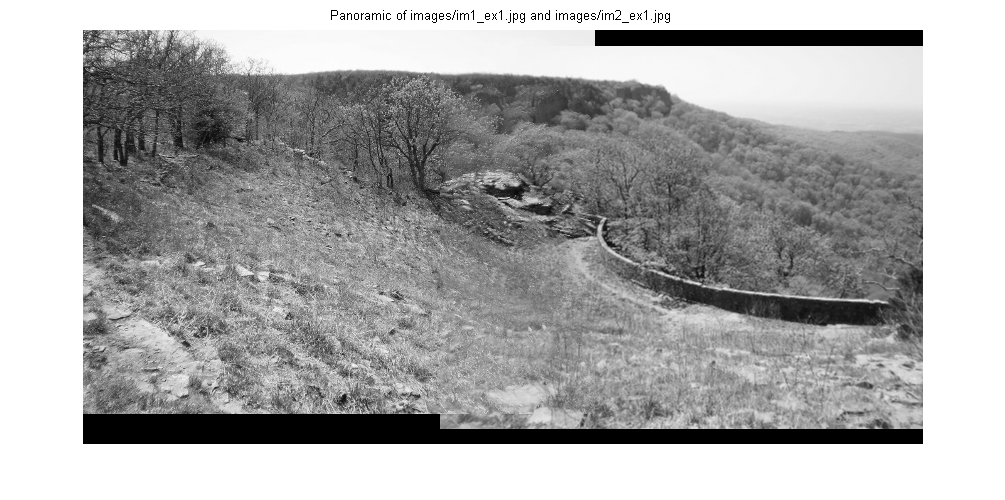
\includegraphics[width=\textwidth]{./img/ex2/panoramic1.png}
	\caption{Panoramic created from first example}
	\label{fig:panoramic1}
\end{figure}

\begin{figure}[htb]
	\centering
		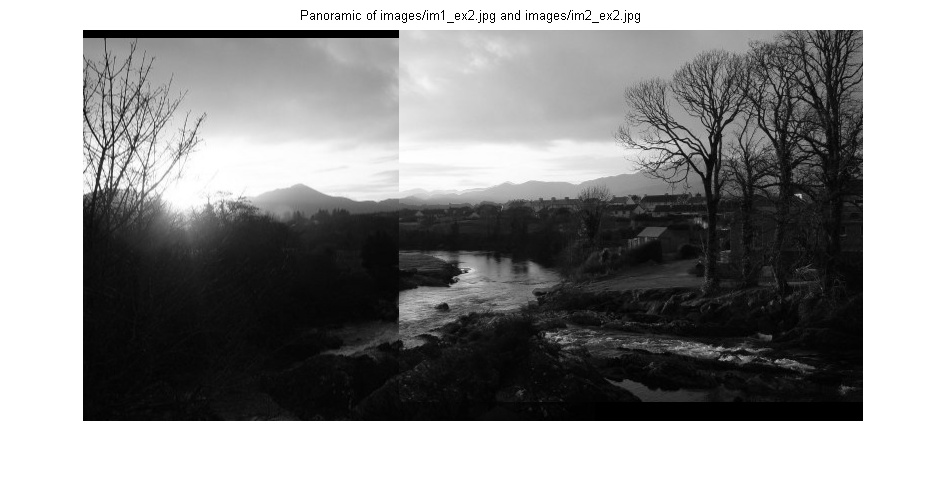
\includegraphics[width=\textwidth]{./img/ex2/panoramic2.png}
	\caption{Panoramic created from second example}
	\label{fig:panoramic2}
\end{figure}

\begin{figure}[htb]
	\centering
		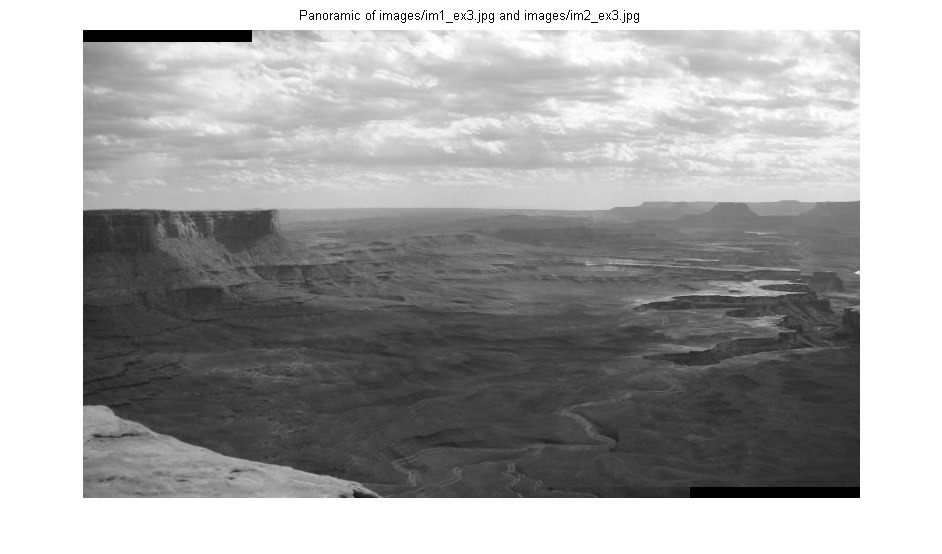
\includegraphics[width=\textwidth]{./img/ex2/panoramic3.png}
	\caption{Panoramic created from third example}
	\label{fig:panoramic3}
\end{figure}

\begin{figure}[htb]
	\centering
		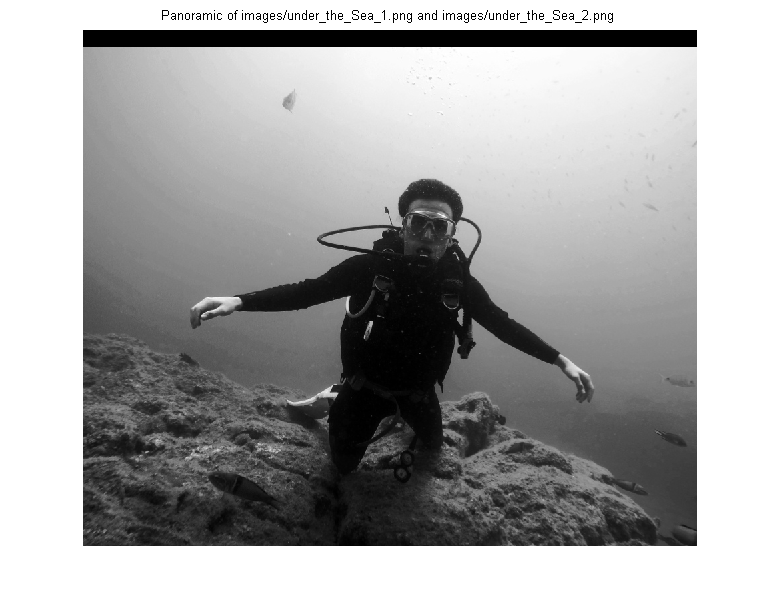
\includegraphics[width=\textwidth]{./img/ex2/panoramic4.png}
	\caption{Panoramic created from fourth example (custom example)}
	\label{fig:panoramic4}
\end{figure}

We can see that the results in all cases are quite acceptable. The second
example is the one with the most perceptible transition from one half
of the image to the other due to small changes in the brightness, the
misalignment of the clouds and the non-still waters. In the rest of
the cases, the transition is smooth enough to be overlooked by all but
the eagle-eyed viewer.